\documentclass[12pt]{article}
\usepackage[utf8]{inputenc}
\usepackage[T1]{fontenc}
\usepackage[USenglish]{babel}
\usepackage{a4wide}
\usepackage{relsize}
\usepackage{placeins}
\usepackage{rotating}
\usepackage{mathtools}
\usepackage{lmodern}
\usepackage{color}
\usepackage{url}
\usepackage{hyperref}

\title{\textbf{Multi-Camera Self-Calibration}\\{\large Technical report}}
\author{Wojciech Szęszoł\thanks{\textit{e-mail}:\texttt{ciechowoj@gmail.com}}}
\date{Wrocław, Oct 3, 2016}


\newcommand{\ds}[0]{\displaystyle}
\newcommand{\ml}[0]{\mathlarger}

\newcommand{\smatheq}[1] {
    \scalebox{0.60}{
        \begin{minipage}{2.1\linewidth}
          \begin{equation}
          \label{eq:vertical}
                #1
            \end{equation}
        \end{minipage}
    }
}

\newcommand{\matheq}[1] {
$$
\begin{aligned}
#1
\end{aligned}
$$
}

\newcommand{\nmatheq}[1] {
\begin{equation}
\begin{aligned}
#1
\end{aligned}
\end{equation}
}

\newcommand{\lmatheq}[1] {
    \scalebox{1.2}{
        \begin{minipage}{0.744\linewidth}
            \begin{align*}
                #1
            \end{align*}
        \end{minipage}
    }
}

\newcommand{\bmatheq}[1] {
    \scalebox{1.0}{
        \begin{minipage}{0.98\linewidth}
            \begin{align*}
                #1
            \end{align*}
        \end{minipage}
    }
}

\newcommand{\hmatheq}[1] {
\[ \scalebox{2}{$#1$} \]
}

\newcommand{\code}[1]{\texttt {\noindent\ignorespaces #1}}

\newcommand{\blist}[1] {
\begin{itemize}
#1
\end{itemize}
}

\newcommand{\rarrow}{\rightarrow}
\newcommand{\larrow}{\leftarrow}
\newcommand{\lrarrow}{\leftrightarrow}
\newcommand{\norm}[1]{\left\lVert#1\right\rVert}

\newcommand{\xa}[1] {\left< #1 \right> }
\newcommand{\xb}[1] {\left{ #1 \right} }
\newcommand{\xp}[1] {\left( #1 \right)}
\newcommand{\xs}[1] {\left[ #1 \right]}


\newcommand{\E}[1] {E \left[ #1 \right]}
\newcommand{\xE}[1] {E \left[ #1 \right]}
\newcommand{\xsum}[2] {\sum\limits_{#1}^{#2}}
\newcommand{\xint}[2] {\int_{#1}^{#2}}
\newcommand{\xd}[1] {\, d#1}

\newcommand{\omegai}[0] {\omega_i}
\newcommand{\omegao}[0] {\omega_o}

\newcommand{\red}[1] {\begingroup\color{red}#1\endgroup}

\makeatletter
    \newenvironment{withoutheadline}{
        \def\beamer@entrycode{\vspace*{-\headheight}}
    }{}
\makeatother


\newcommand{\imageframe}[2]{
    \begin{withoutheadline}
    \begin{frame}
        \centerline{\includegraphics[width=#2\textwidth]{#1}}
        \begin{flushright}
        [Qin 2015]
        \end{flushright}
    \end{frame}
    \end{withoutheadline}
}

%\newcommand{\cev}[1]{\reflectbox{\ensuremath{\vec{\reflectbox{\ensuremath{#1}}}}}}

\makeatletter
\DeclareRobustCommand{\cev}[1]{%
  \mathpalette\do@cev{#1}%
}
\newcommand{\do@cev}[2]{%
  \fix@cev{#1}{+}%
  \reflectbox{$\m@th#1\vec{\reflectbox{$\fix@cev{#1}{-}\m@th#1#2\fix@cev{#1}{+}$}}$}%
  \fix@cev{#1}{-}%
}
\newcommand{\fix@cev}[2]{%
  \ifx#1\displaystyle
    \mkern#23mu
  \else
    \ifx#1\textstyle
      \mkern#23mu
    \else
      \ifx#1\scriptstyle
        \mkern#22mu
      \else
        \mkern#22mu
      \fi
    \fi
  \fi
}

\makeatother

% http://tex.stackexchange.com/questions/114321/extensible-vec-instead-of-overrightarrow
\makeatletter
\newcommand{\lvec}[1]{%
  \vbox{\m@th \ialign {##\crcr
  \vectfill\crcr\noalign{\kern-\p@ \nointerlineskip}
  $\hfil\displaystyle{#1}\hfil$\crcr}}}
\def\vectfill{%
  $\m@th\smash-\mkern-7mu%
  \cleaders\hbox{$\mkern-2mu\smash-\mkern-2mu$}\hfill
  \mkern-7mu\raisebox{-4.45pt}[\p@][\p@]{$\mathord\mathchar"017E$}$}

\renewcommand{\lvec}{%
  \mathpalette {\overarrow@\vectfill@}}
\def\vectfill@{\arrowfill@\relbar\relbar{\raisebox{-4.45pt}[\p@][\p@]{$\mathord\mathchar"017E$}}}

\renewcommand{\lvec}{%
  \mathpalette {\overarrow@\vectfillb@}}
\newcommand{\vecbar}{%
  \scalebox{1}[0.86]{$\relbar$}}
\def\vectfillb@{\arrowfill@\vecbar\vecbar{\raisebox{-4.69pt}[\p@][\p@]{$\mathord\mathchar"017E$}}}
\makeatother

\begin{document}

\maketitle

\thispagestyle{empty}
\newpage

\section{Introduction}

There are many applications for multi-camera systems in the computer industry. Motion capture studios use multiple cameras for tracking special markers. Multiple
cameras are used to track the position headsets in emerging VR technology. The systems of
cameras are becoming indispensable piece of modern technology.

The majority of such systems require some kind of calibration before being
ready to provide target functionality. Calibration is the process of
estimating position and orientation of cameras with respect to each other
and to surrounding environment and sometimes the parameters of cameras itself.

There are multiple ways to do the calibration. One way is to exploit the
geometrical relationships between inputs from the cameras itself. This report
describes a simplified implementation of algorithm presented in "A Convenient
Multi-Camera  Self-Calibration for Virtual Environments" paper by Svoboda et al.
\cite{svoboda05}.

The algorithm uses correspondence and position of points seen from different
cameras of the system. The points are created by waving some bright object
(like modified laser pointer or diffuse LED diode). The bright object will be
called a pointer in the rest of this report. A full version of the algorithm is
very robust, it is immune for measurement noise and significant amount of
occlusions (the pointer doesn't have to be visible from all cameras at once).

Images of the pointer seen from different cameras can be easily matched to each
other (if cameras are synchronized, the images seen at the same frame are the
matching ones). It is relatively easy to detect the pointer position on the
image from the camera as it has very high intensity in comparison to the
environment.

\section{Algorithm Outline}

The 3D positions of the pointer across different time moments (on different frames
from the camera  capture) forms a point cloud. The pixel locations of the points
from the point cloud will be  called image projections. Let $q_i^j$ be the
image projection of i-th point from j-th  camera. The image projection has form
$q_i^j = \begin{bmatrix} x_i^j & y_i^j & 1 \end{bmatrix}^T$, where $x_i^j$ and
$y_i^j$ are  pixel coordinates in the system, which has the origin at the center of
the image and which has x and y axes pointing left and up respectively. We can
arrange all such image projections in a   matrix $W$ called measurement matrix.
Some of the fields in the measurement matrix may be empty due to occlusions (a
point can be invisible from the given camera, occluded by some other object or the
procedure that localized the bright spot on the image may fail and not report
any location). Equation~\ref{eq:w1} shows the measurement matrix with some
elements missing (marked as $\times$).

\nmatheq {
    \label{eq:w1}
    W =
    \begin{bmatrix}
        x_0^0  & x_1^0  & x_2^0  & x_3^0  & x_4^0  & x_5^0  & x_6^0  & \hdots & x_n^0 \\
        y_0^0  & y_1^0  & y_2^0  & y_3^0  & y_4^0  & y_5^0  & y_6^0  & \hdots & y_n^0 \\
        1      & 1      & 1      & 1      & 1      & 1      & 1      & \hdots & 1 \\
        x_0^1  & x_1^1  & x_2^1  & \times & x_4^1  & x_5^1  & \times & \hdots & x_n^1 \\
        y_0^1  & y_1^1  & y_2^1  & \times & y_4^1  & y_5^1  & \times & \hdots & y_n^1 \\
        1      & 1      & 1      & \times & 1      & 1      & \times & \hdots & 1 \\
        \vdots & \vdots & \vdots & \vdots & \vdots & \vdots & \vdots &        & \vdots \\
        x_0^m  & x_1^m  & \times & x_3^m  & x_4^m  & x_5^m  & x_6^m  & \hdots & x_n^m \\
        y_0^m  & y_1^m  & \times & y_3^m  & y_4^m  & y_5^m  & y_6^m  & \hdots & y_n^m \\
        1      & 1      & \times & 1      & 1      & 1      & 1      & \hdots & 1 \\
    \end{bmatrix}
}

Lets consider a single point $Q_i$ and a camera matrix $P^j$. Equation
\ref{eq:projection} defines a rescaled image projection of the point $Q_i$ for
the camera $P^j$.

\nmatheq {
    \label{eq:projection}
    \lambda_i^j q_i^j =
    \begin{bmatrix}
        \lambda_i^j x_i^j \\
        \lambda_i^j y_i^j \\
        \lambda_i^j
    \end{bmatrix}
    = P_j Q_i
}

The factors $\lambda_i^j$ are called projective depths. The image projections in
the measurement matrix, that comes as the input of the algorithm have the projective
depths divided out. The measurement matrix $\hat{W}$ with known projective
depths will be called a rescaled measurement matrix. The rescaled measurement
matrix has rank four, if no noise is present. If the projective depths were
known and there was no holes in the rescaled measurement matrix, it could be
factorized into the set of camera matrices $\hat{P}$ and the set of point locations
$\hat{Q}$.  However, the factorization would be only up to some projective
transformation. An additional  Euclidean stratification step is needed to
recover $P$ and $Q$ in the Euclidean space. Equation ~\ref{eq:w2} presents factorization of the rescaled measurement matrix.

\nmatheq {
    \label{eq:w2}
    \hat{W} &= \hat{P}\hat{Q} = \\
    \begin{bmatrix}
        \lambda_0^0 x_0^0  & \lambda_1^0 x_1^0  & \lambda_2^0 x_2^0  & \lambda_3^0 x_3^0  & \hdots & \lambda_n^0 x_n^0 \\
        \lambda_0^0 y_0^0  & \lambda_1^0 y_1^0  & \lambda_2^0 y_2^0  & \lambda_3^0 y_3^0  & \hdots & \lambda_n^0 y_n^0 \\
        \lambda_0^0        & \lambda_1^0        & \lambda_2^0        & \lambda_3^0        & \hdots & \lambda_n^0   \\
        \lambda_0^1 x_0^1  & \lambda_1^1 x_1^1  & \lambda_2^1 x_2^1  & \lambda_3^1 x_3^1  & \hdots & \lambda_n^1 x_n^1 \\
        \lambda_0^1 y_0^1  & \lambda_1^1 y_1^1  & \lambda_2^1 y_2^1  & \lambda_3^1 y_3^1  & \hdots & \lambda_n^1 y_n^1 \\
        \lambda_0^1        & \lambda_1^1        & \lambda_2^1        & \lambda_3^1        & \hdots & \lambda_n^1   \\
        \vdots             & \vdots             & \vdots             & \vdots             &        & \vdots \\
        \lambda_0^m x_0^m  & \lambda_1^m x_1^m  & \lambda_2^m x_2^m  & \lambda_3^m x_3^m  & \hdots & \lambda_n^m x_n^m \\
        \lambda_0^m y_0^m  & \lambda_1^m y_1^m  & \lambda_2^m y_2^m  & \lambda_3^m y_3^m  & \hdots & \lambda_n^m y_n^m \\
        \lambda_0^m        & \lambda_1^m        & \lambda_2^m        & \lambda_3^m        & \hdots & \lambda_n^m   \\
    \end{bmatrix}
    &=
    \begin{bmatrix}
        \hat{P}^0 \\
        \hat{P}^1 \\
        \vdots \\
        \hat{P}^m \\
    \end{bmatrix}
    \cdot
    \begin{bmatrix}
        \hat{Q_0} & \hat{Q_1} & \hat{Q_2} & \hat{Q}_3 & \hdots & \hat{Q_n} \\
    \end{bmatrix}
}

If the real world locations of some (at least three which are not co-linear)
points $Q_i$ are known, recovered structures can be aligned with real world
frame of reference (otherwise the scale, rotation and translation of recovered
structures are completely arbitrary). The outline of the algorithm is (each step will be described in the subsequent sections):

\begin{enumerate}
\item Fill gaps in measurement matrix.
\item Recover projective depths.
\item Factorize rescaled measurement matrix.
\item Perform Euclidean stratification.
\item Align recovered structures with real world frame of reference.
\end{enumerate}

The steps 1. and 2. have to be done together, as explained in the next section,
they need to be repeated several times to recover the rescaled measurement matrix from
the partial measurement matrix.

\section{Filling the gaps}
\subsection{Recovering projective depths}

Before trying to fill missing elements, the projective depths of known points
need to be computed. Observe, that any column and any triple of rows associated
with some camera matrix  $P_j$ of the rescaled measurement matrix can be
multiplied with nonzero scalar without changing the information the rescaled
measurement matrix contains (e.g. the camera parameters or the point
locations). The multiplication of a column is canceled by the fact that point
locations are in homogeneous coordinates and $w$ component accommodates the
scaling. Camera matrices can accommodate the scaling in similar manner. That
means projective depths can be fixed for single triple of rows and the rest of
the depths can be calculated with respect to that fixed row. To compute
projective depths of some other row $k$ with respect to the fixed one $j$, the
fundamental matrix $F^{jk}$ and the left epipole $e^{jk}$ need to be computed
\cite{sturm96}. It can be done with the eight point algorithm \cite{hartley95}
(there are   also seven and five point variations \cite{stewenius06}, however
my implementation uses only    the simplest, eight point one), then the
projective depths can be computed according to equation:

\nmatheq {
    \lambda_i^k = \frac{(e^{jk} \times q_i^k) \cdot (F^{jk} q_i^j)}{\norm{e^{jk} \times q_i^k}^2} \lambda_i^j
}

The function that does the above is called \code{recover\_projective\_depths}, it
takes two $3 \times n$ matrices \code{A} and \code{B}. It assumes that
projective depths in \code{A} are known and returns a new matrix that is copy of
\code{B} with projective depths filled in. The fundamental matrix and the left
epipole are computed with functions \code{fundamental\_matrix} and
\code{left\_epipole} respectively. For numerical stability
\code{fundamental\_matrix} normalizes the image projections. There is also
another function \code{recover\_all\_projective\_depths} takes a $3m \times n$
matrix and computes all projective depths.

\subsection{Filling missing elements}

A property of the rescaled measurement matrix that allows to recover its unknown
elements is that in noise free conditions it has rank 4. That means its column
space is four dimensional. If the basis $\mathcal{B}$ of that space is known,
every other column can be expressed as linear combination of the vectors from
that basis. The only condition is the column with missing elements are required
to have at least four elements known (as the linear combination coefficients
have to be computed first). In practice, four elements means at least two image
projections. First four element tuples $A_t$ of columns are sampled from the
rescaled measurement matrix. It is not guaranteed that any of them spans the
basis $\mathcal{B}$. However, the intersection of the subspaces spanned by them
should span $\mathcal{B}$. That is given set $\mathcal{B}_t$ of linear subspaces
generated by tuples of columns $A_t$, $\mathcal{B}$ can be computed as
$\mathcal{B} = \bigcap_{t \in T} \! \mathcal{B}_t = (Span_{t \in T}
\mathcal{B}_t^\bot)^\bot$.  However, the tuples $A_t$ may lack some of their
elements. In \cite{svoboda04} a way to extend incomplete tuples $A_t$ to
extended tuples $B_t$, that can take part in further processing was shown. A
tuple $B_t$ can be created from $A_t$ by replacing all of the unknown elements
with $0$ and adding some extra columns for the incomplete ones. For  every
column that doesn't have a projective depth, the extra column with zeros and
known  image projections should be added. If a column doesn't contain given
point at all, a triple of columns with the standard basis spanning the
dimensions of the unknown point should be added. Equation~\ref{eq:extendAt}
illustrates it.

\nmatheq {
    \label{eq:extendAt}
    A_t &=
    \begin{bmatrix}
        \lambda_1^1 q_1^1 & \lambda_2^1 q_2^1 & \times            & \lambda_4^1 q_4^1 \\
        \lambda_1^2 q_1^2 & \lambda_2^2 q_2^2 & \lambda_3^2 q_3^2 & \lambda_4^2 q_4^2 \\
        ? q_1^3           & \lambda_2^3 q_2^3 & \lambda_3^3 q_3^3 & \lambda_4^3 q_4^3 \\
        \vdots            & \vdots            & \vdots            & \vdots            \\
        \lambda_1^m q_1^m & \lambda_2^m q_2^m & \lambda_3^m q_3^m & \lambda_4^m q_4^m \\
    \end{bmatrix}
    \rarrow \\
    B_t &=
    \begin{bmatrix}
        \lambda_1^1 q_1^1 & 0      &\lambda_2^1 q_2^1 & 0                 & \begin{bmatrix} 1 \\ 0 \\ 0 \end{bmatrix} & \begin{bmatrix} 0 \\ 1 \\ 0 \end{bmatrix} & \begin{bmatrix} 0 \\ 0 \\ 1 \end{bmatrix} & \lambda_4^1 q_4^1 \\
        \lambda_1^2 q_1^2 & 0      &\lambda_2^2 q_2^2 & \lambda_3^2 q_3^2 & 0                                         & 0                                         & 0                                         & \lambda_4^2 q_4^2 \\
        0                 & q_1^3  &\lambda_2^3 q_2^3 & \lambda_3^3 q_3^3 & 0                                         & 0                                         & 0                                         & \lambda_4^3 q_4^3 \\
        \vdots            & \vdots &\vdots            & \vdots            & \vdots                                    & \vdots                                    & \vdots                                    & \vdots            \\
        \lambda_1^m q_1^m & 0      &\lambda_2^m q_2^m & \lambda_3^m q_3^m & 0                                         & 0                                         & 0                                         & \lambda_4^m q_4^m \\
    \end{bmatrix}
}

The generators $B_t^\bot$ of $\mathcal{B}_t^\bot$ can be computed by taking SVD
of $B_t$: $[u, s, v] = svd(B_t)$. The generators are equal to $u[:, d:]$
(the indexing operator $[]$ uses the Python convention), where $d$ is dimension of
$\mathcal{B}_t$, which is number of nonzero entries in $s$. To compute $(Span_{t
\in T} \mathcal{B}_t^\bot)^\bot$, one needs to take $[u, s, v] = svd([B_1^\bot
B_2^\bot \dots B_t^\bot])$ and $(Span_{t \in T} \mathcal{B}_t^\bot)^\bot$ is
equal to $u[:, -4:]$. The detailed description how to recover the column space
can be found in \cite{jacobs99} and \cite{svoboda04}. The function that computes
the rank four column space in the associated program is called
\code{rank\_four\_column\_space}. It takes the rescaled measurement matrix, and
returns a new matrix with four columns that are basis for its column space.

\subsection{Iterative approach}

To recover all of the missing image projections, the
steps just described needs to be applied iteratively. At first the triple of
rows that has the greatest number of elements filled is found, lets call it the
fixed triple. Then all triples that have at least eight elements known in common
with the fixed triple are gathered (the restriction imposed by the eight point
algorithm). Then the sub-matrix from all of the collected triples is created and
the projective depths for known projections are estimated. The next step is to
compute the basis of column space and use it to fill the missing elements. The
process is repeated until all the gaps are filled. The function responsible for
the process is \code{reconstruct\_missing\_data}. It takes a measurement matrix
\code{W} and returns its copy with gaps filled and the projective depths
computed.

\section{Factorization of Measurement Matrix}

Having the projective depths
recovered, rescaled measurement matrix $W$ can be factorized to set of camera
matrices $\hat{P}$ and point positions $\hat{Q}$. The factorization can only by
done up to some unknown projective transformation, but this issue will be fixed
in the next step. As rescaled measurement matrix is rank 4 matrix, it can be
factorized with SVD. However, before factorization it should be balanced to
provide better stability of SVD (\cite{sturm96}). To balance the matrix, columns
are rescaled, so that $\forall_{1 \leq i \leq n} \sum_{j=1}^m \left( (\lambda
_i^j x_i^j)^2 + (\lambda _i^j y_i^j)^2 + (\lambda _i^j)^2 \right)~=~1$ and
triples of rows are rescaled, so that $\forall_{1 \leq j \leq m} \sum_{i=0}^n
\left( (\lambda _i^j x_i^j)^2 + (\lambda _i^j y_i^j)^2 + (\lambda _i^j)^2
\right) = 1$. The~balancing is done with \code{balance\_measurement\_matrix}
function. In (\cite{sturm96}) it is suggested to repeat balancing until the
measurement matrix  changes, however in my implementation number of balancing
steps is fixed to some constant.

After balancing, the matrix can be factorized with SVD. Equation~\ref{eq:rank4}
illustrates it. As factorization of $s$ can be arbitrary, it is factorized by
taking square root. The factorization is a part of the
\code{factor\_measurement\_matrix} procedure.

\nmatheq {
    \label{eq:rank4}
    u, s, v &= svd(\hat{W}) \\
    \hat{P} &= u[:, :4] \cdot \sqrt{s} \\
    \hat{Q} &= \sqrt{s} \cdot v[:4, :] \\
}


\section{Euclidean Stratification}

The matrices $\hat{P}$ and $\hat{Q}$ are recovered up to some unknown projective
transformation. An arbitrary projective transformation matrix $HH^{-1}$ can be inserted
in-between $\hat{P}$ and $\hat{Q}$ and factorization still will be correct.

\nmatheq{
    W = \hat{P}HH^{-1}\hat{Q} = PQ
}

To upgrade the projective factorization to the Euclidean one, the constraints on
the rescaled measurement matrix $W$ and the camera matrix $P$ needs to be
imposed. The first set of constraints puts the origin of the coordinate system
to the centroid of yet unknown points. The  second constraints uses properties
of the camera matrices (an orthogonality of rotation matrix   axes). The
constraints give a raise to set of equations, which if solved gives a matrix
that   changes recovered structures to Euclidean ones. The details can be found
in \cite{svoboda05}   and \cite{han00}. At the end of the document, the
equations~\ref{eq:b},~\ref{eq:Q} and  ~\ref{eq:vertical} for $b$ and $Q$ for
single camera matrix are given for reference (the   notation from
\cite{svoboda05} is used). They can be extended to full system by stacking them
together. The function \code{factor\_measurement\_matrix} solves the equations
and returns   stratified matrix.

\section{Fixing Camera Matrices}

As the triples of rows associated with given cameras can be multiplied by any
nonzero scalar, there is ambiguity in recovered cameras. The z-axis of the
camera may be reversed. To fix that a simple heuristic is used. The number of
points visible in front of camera and in the back of it is counted and if the
number of points visible at the rear side of camera is greater that at  the
front, the z-axis is reversed. \code{resolve\_camera\_ambiguity} function is
intended for  that purpose.

\section{Alignment with World}

To align recovered structures with the real world frame of reference the
positions of at least three point in real world that are not lying on the same line
are needed. In the face of noise additional locations will improve the accuracy
though. A system of linear equations can be created and solved with SVD to
compute a matrix that transforms the structures to the world coordinate system.
In my implementation \code{find\_frame\_of\_reference} is the function which
does that.

\newpage

\section{Dissecting the Camera Matrix}

After successful factorization, to recover intrinsic and extrinsic camera
parameters, the camera matrices needs to be factorized out. The function that
does the job is called \code{decompose}, it takes a camera matrix and returns
tuple $(K, R, T)$ with the matrix of intrinsic parameters, the rotation and the translation
vector. First the $P$ matrix is factorized with the RQ algorithm $\bar{K},
\bar{R} = rq(P[:3, :3])$. This factorization is slightly ambiguous and following
steps \cite{simek12} are carried out to fix it (the fixed matrices will be called $\bar{K}'$~and~$\bar{R}'$):

\begin{enumerate}
\item If $\bar{K}_{00}$ is negative multiply both the first column of $\bar{K}$ and first row
of $\bar{R}$ by $-1$.
\item If $\bar{K}_{11}$ is negative multiply both the second column of $\bar{K}$ and second row
of $\bar{R}$ by $-1$.
\item If $\bar{K}_{22}$ is positive (cameras from my implementation has reversed z-axis)
multiply both the third column of $\bar{K}$ and third row of $\bar{R}$ by $-1$.
\item If determinant of $\bar{R}$ is negative multiply the whole matrix by $-1$.
\end{enumerate}

Then translation is computed as $T = (\bar{K}' \cdot (-\bar{R}'))^{-1} \cdot
P[:3, 3]$. The  last thing is to remove scaling from $\bar{K}$: $K =
\dfrac{\bar{K}''}{\bar{K}'[2,2]}$.

\section{Experiments}

Several experiments were conducted, on two test scenes, including one with real
data. Figure~\ref{fig:artificial} presents the artificial scene. It consist of
10 cameras, the test points were randomly drawn from inside of the sphere. The
points were transformed with the camera matrices, to obtain their pixels
positions in the coordinate systems of the respective cameras. Then random noise was
added to each of the pixel positions. Given a pixel position $p = (p_x, p_y)$, the
new pixel position $p' = (p_x', p_y')$ with the noise added is $p_x' = p_x + (2
\cdot \xi - 1) \cdot \varepsilon$, where $\xi$ is a standard uniform random
variable ($\xi \in [0, 1)$), and $\varepsilon$ controls an amount of the noise added (the
same~for~$y$).

\begin{figure}[!ht]
\centering
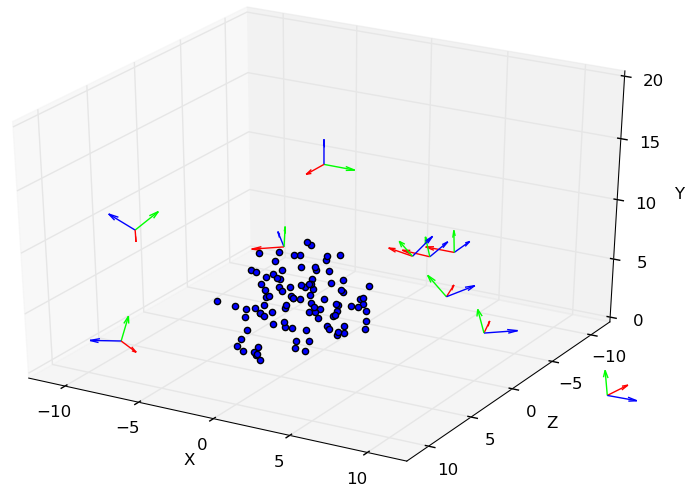
\includegraphics[scale=0.5]{artificial.png}
\caption{The arrangement of the cameras in artificial scene.}
\label{fig:artificial}
\end{figure}

In a part of the tests, some of the pixel positions were erased to test if my
implementation can handle the occlusions. The results are summarized in the
table~\ref{tab:artificial}. The RMS error refers to the random mean square root
error between the reference and recovered camera positions. To compute the error, the camera positions were interpreted as a flat array (see numpy's \code{ravel}). The "missing" column
contains the fraction of the pixel positions erased.

\begin{table}[!ht]
\centering
\begin{tabular}{|l|r|r|r|r|r|r|}
\hline
\multicolumn{1}{|c}{ \bfseries name} &
\multicolumn{1}{|c}{ \bfseries cameras} &
\multicolumn{1}{|c}{ \bfseries points} &
\multicolumn{1}{|c}{ \bfseries missing} &
\multicolumn{1}{|c}{ \bfseries noise ($\varepsilon$)} &
\multicolumn{1}{|c|}{\bfseries RMS error } \\ \hline
\code{testset\_m\_0\_0\_e\_0\_0}      & 10 & 100 & 0.0 & 0.0       & 0.00283 \\ \hline
\code{testset\_m\_0\_1\_e\_0\_0}      & 10 & 100 & 0.1 & 0.0       & 0.00287 \\ \hline
\code{testset\_m\_0\_2\_e\_0\_0}      & 10 & 100 & 0.2 & 0.0       & 0.00275 \\ \hline
\code{testset\_m\_0\_4\_e\_0\_0}      & 10 & 100 & 0.4 & 0.0       & 0.01573 \\ \hline
\code{testset\_m\_0\_8\_e\_0\_0}      & 10 & 100 & 0.8 & 0.0     & not converge \\ \hline
\code{testset\_m\_0\_0\_e\_0\_1}      & 10 & 100 & 0.0 & $10^{-1}$ & 896.504 \\ \hline
\code{testset\_m\_0\_0\_e\_0\_01}     & 10 & 100 & 0.0 & $10^{-2}$ & 15.8931 \\ \hline
\code{testset\_m\_0\_0\_e\_0\_001}    & 10 & 100 & 0.0 & $10^{-3}$ & 19.7910 \\ \hline
\code{testset\_m\_0\_0\_e\_0\_0001}   & 10 & 100 & 0.0 & $10^{-4}$ & 0.04995 \\ \hline
\code{testset\_m\_0\_0\_e\_0\_00001}  & 10 & 100 & 0.0 & $10^{-5}$ & 0.00319 \\ \hline
\code{testset\_m\_0\_1\_e\_0\_001}  & 10 & 100 & 0.1 & $10^{-3}$   & 549.828 \\ \hline
\code{testset\_m\_0\_1\_e\_0\_0001}  & 10 & 100 & 0.1 & $10^{-4}$  & 9.78033 \\ \hline
\end{tabular}
\caption{A summary of the tests carried out with the artificial scene.}
\label{tab:artificial}
\end{table}

% data/testset_m_0_0_e_0_0.csv :  0.00283474054273
% data/testset_m_0_1_e_0_0.csv :  0.00287687828883
% data/testset_m_0_2_e_0_0.csv :  0.002753317657
% data/testset_m_0_4_e_0_0.csv :  0.0157395386403
% data/testset_m_0_0_e_0_1.csv :  896.504346513
% data/testset_m_0_0_e_0_01.csv :  15.8931605235
% data/testset_m_0_0_e_0_001.csv :  19.7910311311
% data/testset_m_0_0_e_0_0001.csv :  0.0499547559616
% data/testset_m_0_0_e_0_00001.csv :  0.00319775979851
% data/testset_m_0_1_e_0_001.csv :  549.828117517
% data/testset_m_0_1_e_0_0001.csv :  9.78033946821

The real data was captured with web and mobile phone cameras. The cameras used
were Nokia Lumia 620 (1280x720), Nokia Lumia 820 (1280x720), Huawei P8 Lite
(1088x1280), Motorola MB860 (1920x1080), Asus K56CB (640x480), Microsoft HD 3000
(640x480), 4WORLD Z200 (640x480) (the values int the parentheses are resolutions).
However, the capture from Motorola had to be discarded due to problems with
synchronization (it was skipping and adding extra frames at random places) and
the capture from Lumia 640 had to be discarded as well (due to lighting conditions). The points were generated by
tracking a bright diffuse white LED. The moment of the LED switching on was used to
synchronize the captures from all of the cameras. A checkerboard with known dimensions was used to capture the frame of reference of the scene. A special tool was written to
extract the pixel positions of the pointer (the source code is in \texttt{sync.py}). Figure~\ref{fig:real} shows the arrangement of cameras on the real scene.

\begin{figure}[ht]
\centering
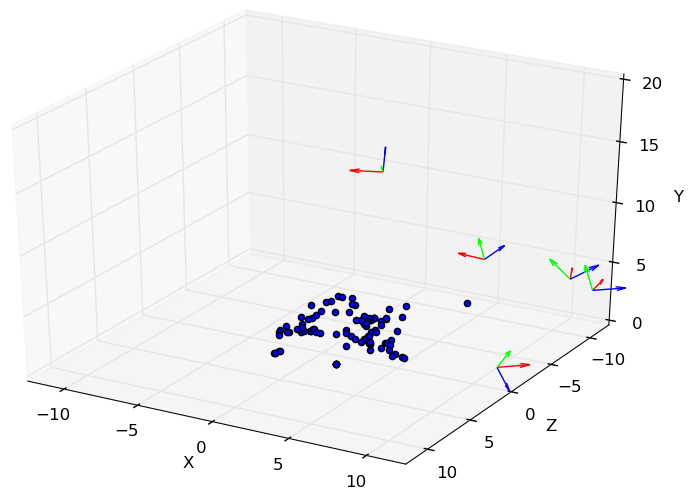
\includegraphics[scale=0.5]{real.png}
\caption{The arrangement of the cameras in real scene.}
\label{fig:real}
\end{figure}


Table~\ref{tab:positions} compares the real positions of the cameras (obtained with a tape measure, with $10cm$ accuracy) with the recovered ones. Table~\ref{tab:real} summarizes the experiment with real scene, a few tests with different degree of missing points were conducted. The "missing" column contains the number of missing pixel positions.

\begin{table}[ht]
\centering
\begin{tabular}{|l|c|c|c|}
\hline
\multicolumn{1}{|c}{\bfseries Camera} &
\multicolumn{1}{|c}{\bfseries Real positions} &
\multicolumn{1}{|c|}{\bfseries Estimated position} \\ \hline
 1 & [16.4, 12.0, -8.2] & [16.4, 8.3, -1.7] \\ \hline
 2 & [18.5, 10.0, -2.8] & [13.5, 7.1, -4.7] \\ \hline
 3 & [5.0, 4.8, -14.7] & [4.6, 3.8, -11.2] \\ \hline
 4 & [16.0, 10.6, 12.4] & [18.2, 9.2,  13.0] \\ \hline
 5 & [-6.3, 10.6, -13.8] & [-2.9, 9.0, -12.2] \\ \hline
\end{tabular}
\caption{The real and recovered camera positions.}
\label{tab:positions}
\end{table}

\begin{table}[!ht]
\centering
\begin{tabular}{|l|r|r|r|r|r|r|}
\hline
\multicolumn{1}{|c}{ \bfseries name} &
\multicolumn{1}{|c}{ \bfseries cameras} &
\multicolumn{1}{|c}{ \bfseries points} &
\multicolumn{1}{|c}{ \bfseries missing} &
\multicolumn{1}{|c|}{\bfseries RMS error } \\ \hline
\code{dataset1}      & 5  & 132 & 0  & 2.92276 \\ \hline
\code{dataset2}      & 5  & 253 & 10 & 3.44128 \\ \hline
\code{dataset3}      & 5  & 263 & 14 & 5.55154 \\ \hline
\code{dataset4}      & 5  & 282 & 21 & 3.40607 \\ \hline
\end{tabular}
\caption{A summary of the tests carried out with the real scene.}
\label{tab:real}
\end{table}

% data/dataset1.csv :  2.92276712426
% data/dataset2.csv :  3.44128694798
% data/dataset3.csv :  5.55154646563
% data/dataset4.csv :  3.40607167903

\begin{figure}[ht]
\centering
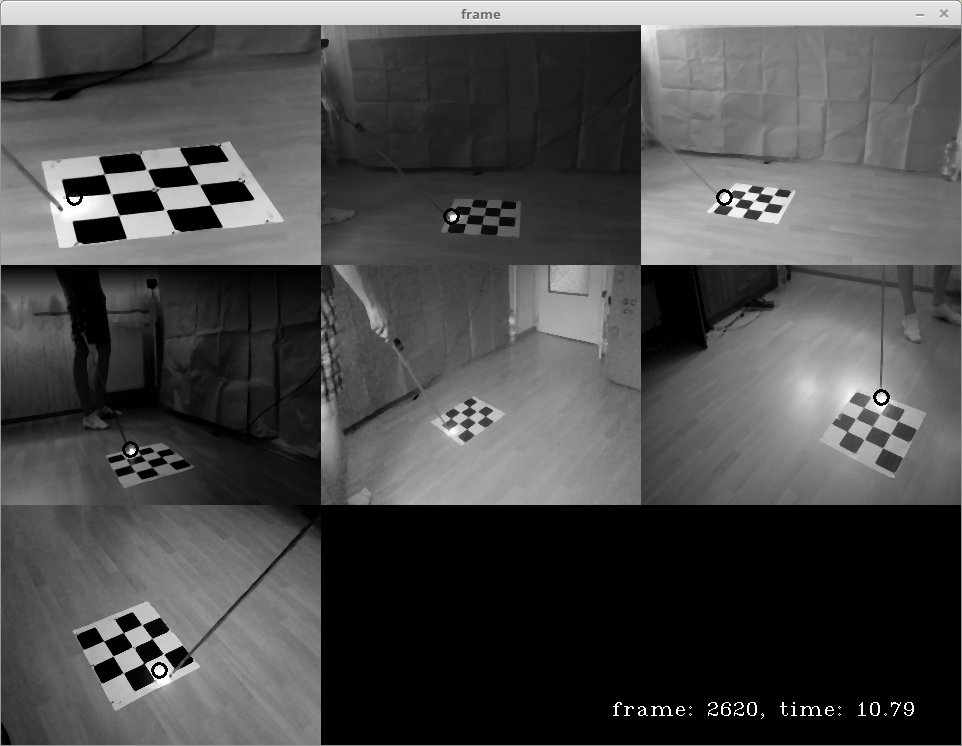
\includegraphics[scale=0.4]{sync.png}
\caption{A screen-shot from the \texttt{sync.py} tool, which was used to synchronize the videos and capture the positions of the pointer (the view from discarded cameras is included).}
\end{figure}

\begin{figure}[ht]
\centering
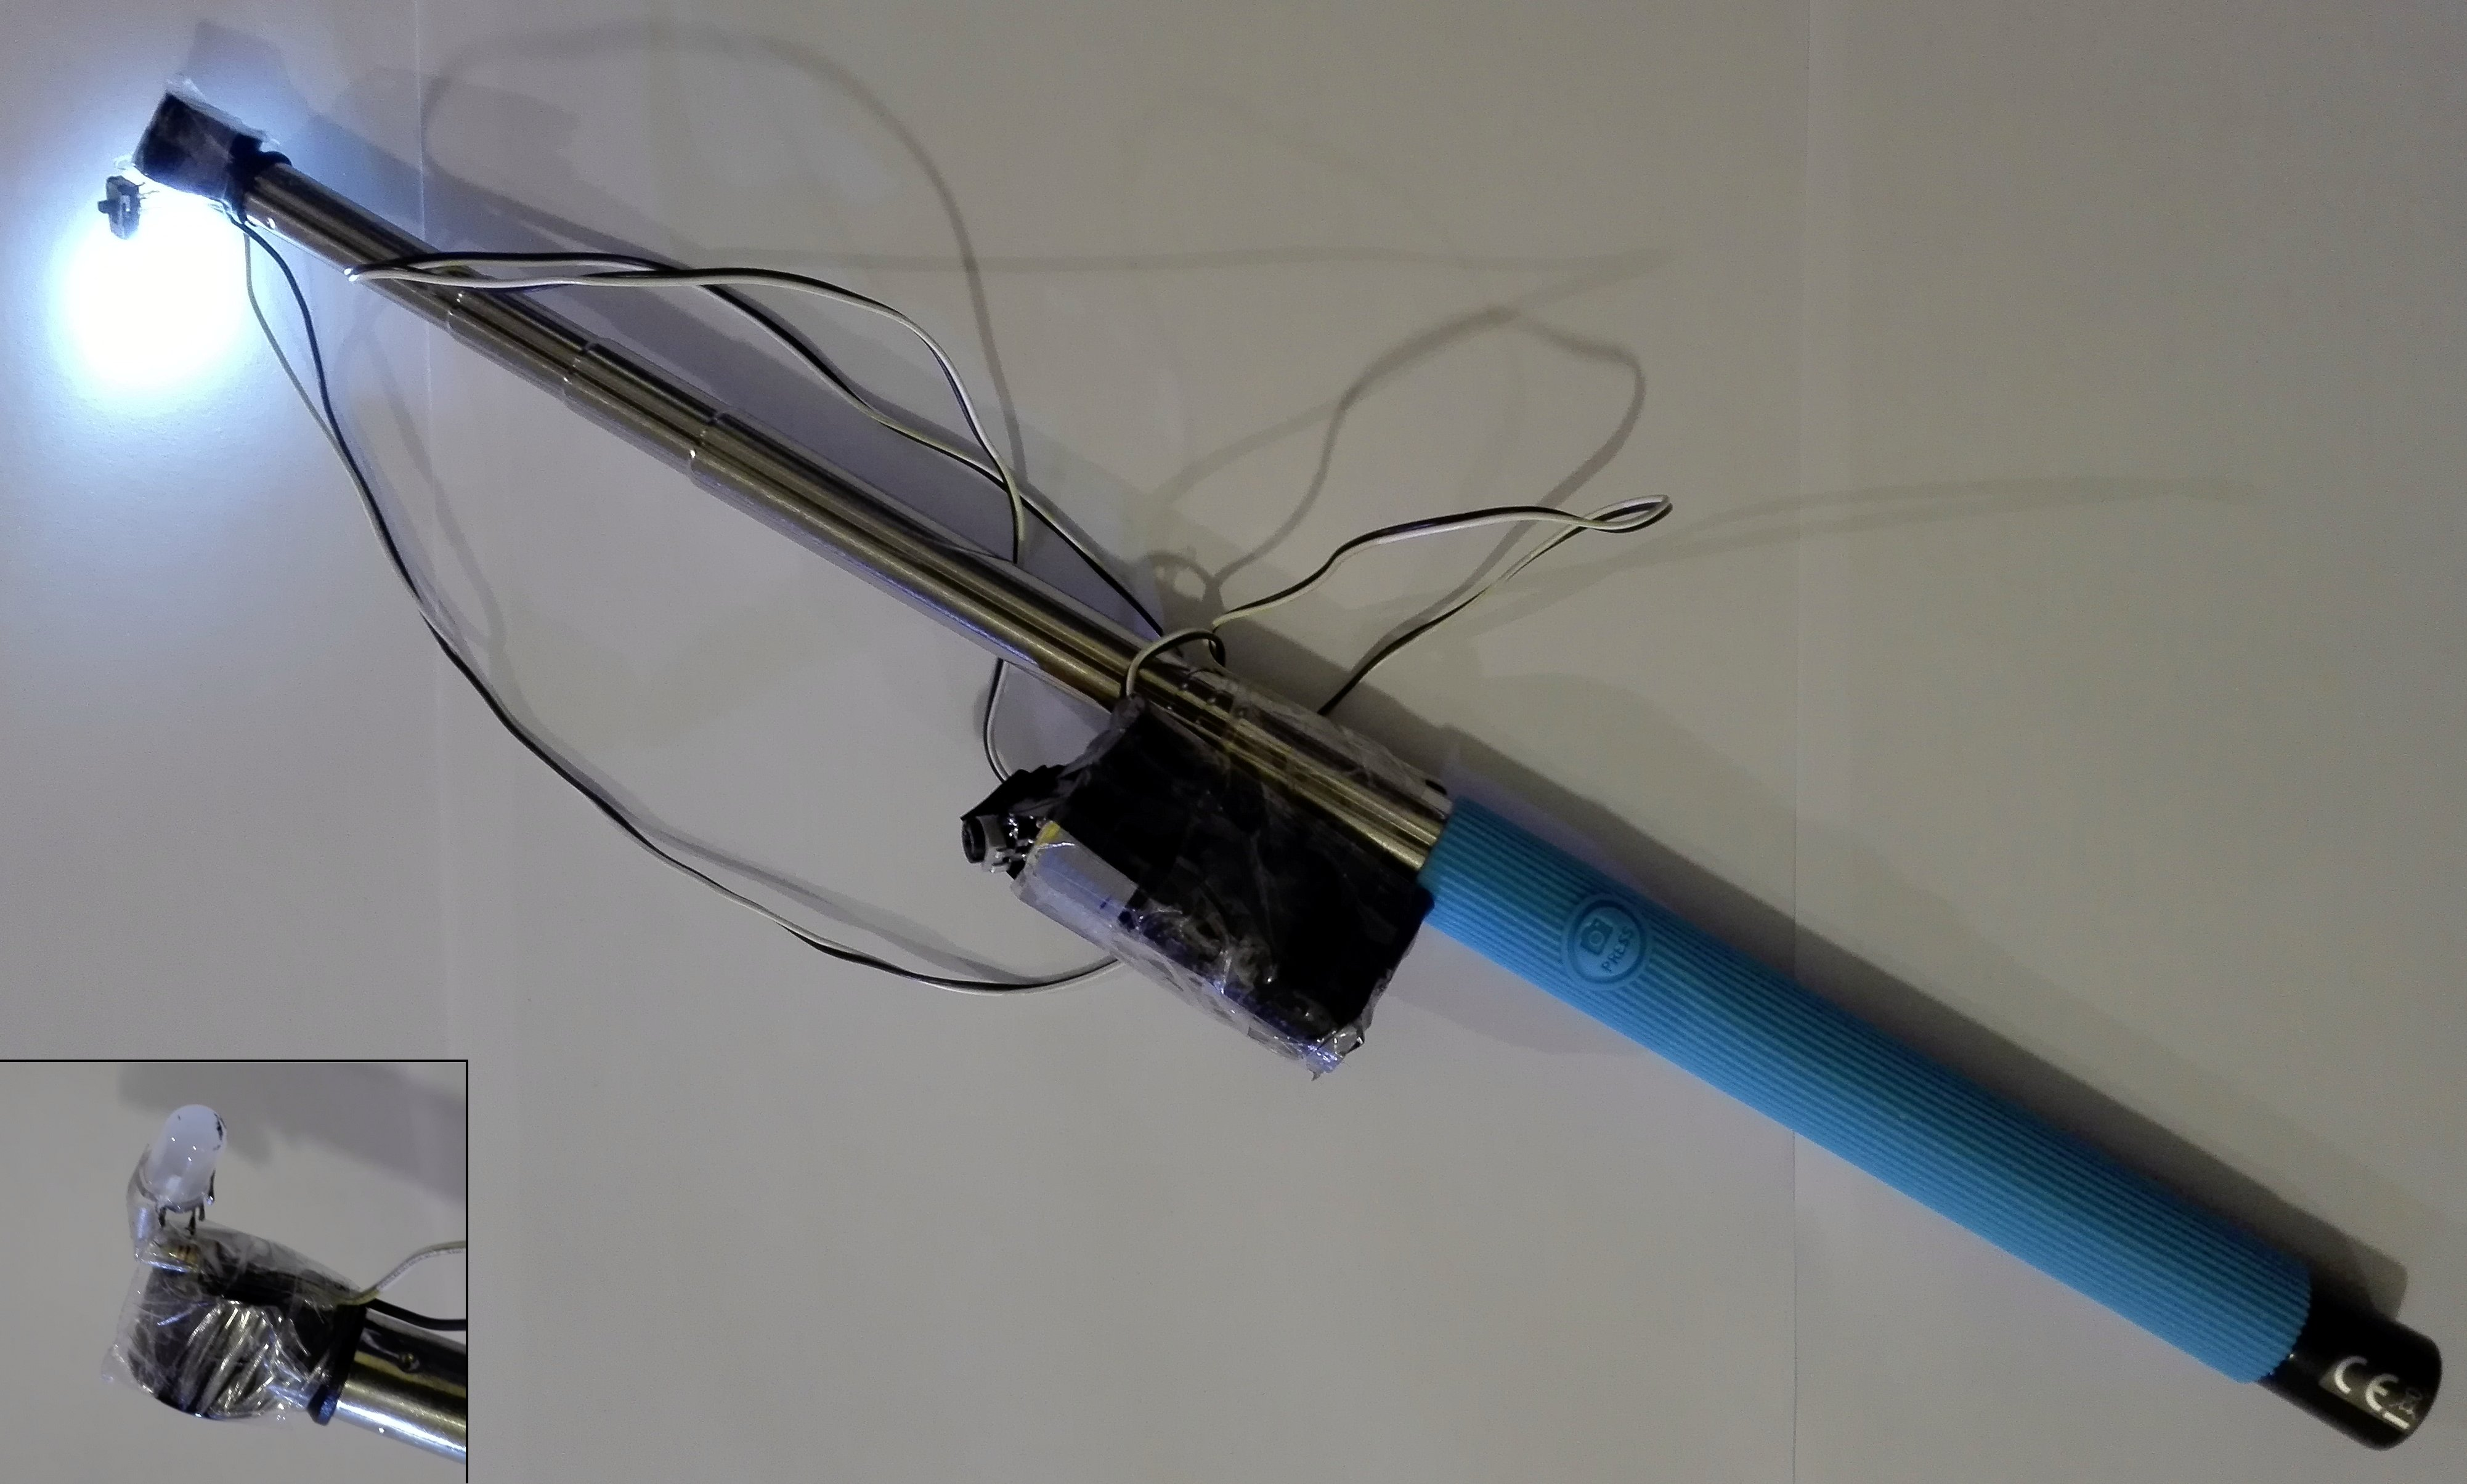
\includegraphics[scale=0.097]{stick.jpg}
\caption{A photo of the "stick" that was used as the pointer.}
\end{figure}

\section{Conclusions}

Implemented algorithm turned out to be quite sensitive to noise. It gives almost
exact results for precise data, but the robustness of the implemented algorithm
quickly diminishes as the error increases. It could have been expected, as some
steps of original implementation \cite{svoboda05} were skipped. The major
problem is the lack of any iterative refinement of the intermediate results (e.g.
optimizing projective structure with Bundle Adjustment, before factorization).
My implementation has not means to handle outliers (the points in real world
experiments were manually selected). The methods applied to sample the columns for
the estimation of the column space basis and to choose the order of computation
of fundamental matrices are very naive in comparison to the ones presented in
the paper. However, as it was experimentally proven, it is robust enough to
recover an approximate structure and motion from the real-world data.

\FloatBarrier

\bibliographystyle{alpha}
\bibliography{main}

The associated code can be found under the following link \url{https://github.com/ciechowoj/calibration} .

\newpage

\section{Equations for Euclidean stratification}

\nmatheq {
    \label{eq:b}
    \begin{dcases}
        (P_z^j)^T b \cdot \frac{T_x^j}{T_z^j} - (P_x^j)^T b &= 0 \\
        (P_z^j)^T b \cdot \frac{T_y^j}{T_z^j} - (P_y^j)^T b &= 0 \\
    \end{dcases} \\
    \begin{dcases}
        P_{z0}^j \frac{T_x^j}{T_z^j} b_x +
        P_{z1}^j \frac{T_x^j}{T_z^j} b_y +
        P_{z2}^j \frac{T_x^j}{T_z^j} b_z +
        P_{z3}^j \frac{T_x^j}{T_z^j} b_w -
        P_{x0}^j b_x +
        P_{x1}^j b_y +
        P_{x2}^j b_z +
        P_{x3}^j b_w &= 0 \\
        P_{z0}^j \frac{T_y^j}{T_z^j} b_x +
        P_{z1}^j \frac{T_y^j}{T_z^j} b_y +
        P_{z2}^j \frac{T_y^j}{T_z^j} b_z +
        P_{z3}^j \frac{T_y^j}{T_z^j} b_w -
        P_{y0}^j b_x +
        P_{y1}^j b_y +
        P_{y2}^j b_z +
        P_{y3}^j b_w &= 0 \\
    \end{dcases} \\
    \begin{dcases}
        \left( P_{z0}^j \frac{T_x^j}{T_z^j} - P_{x0}^j \right) b_x +
        \left( P_{z1}^j \frac{T_x^j}{T_z^j} - P_{x1}^j \right) b_y +
        \left( P_{z2}^j \frac{T_x^j}{T_z^j} - P_{x2}^j \right) b_z +
        \left( P_{z3}^j \frac{T_x^j}{T_z^j} - P_{x3}^j \right) b_w = 0 \\
        \left( P_{z0}^j \frac{T_y^j}{T_z^j} - P_{y0}^j \right) b_x +
        \left( P_{z1}^j \frac{T_y^j}{T_z^j} - P_{y1}^j \right) b_y +
        \left( P_{z2}^j \frac{T_y^j}{T_z^j} - P_{y2}^j \right) b_z +
        \left( P_{z3}^j \frac{T_y^j}{T_z^j} - P_{y3}^j \right) b_w = 0
    \end{dcases} \\
    \begin{bmatrix}
        P_{z0}^j \frac{T_x^j}{T_z^j} - P_{x0}^j & P_{z1}^j\frac{T_x^j}{T_z^j} - P_{x1}^j & P_{z2}^j\frac{T_x^j}{T_z^j} - P_{x2}^j & P_{z3}^j \frac{T_x^j}{T_z^j} - P_{x3}^j \\
        P_{z0}^j \frac{T_y^j}{T_z^j} - P_{y0}^j & P_{z1}^j\frac{T_y^j}{T_z^j} - P_{y1}^j & P_{z2}^j\frac{T_y^j}{T_z^j} - P_{y2}^j & P_{z3}^j \frac{T_y^j}{T_z^j} - P_{y3}^j \\
   \end{bmatrix}
    \cdot
    \begin{bmatrix} b_x \\ b_y \\ b_z \\ b_w \end{bmatrix} = 0
}

\nmatheq {
    \label{eq:Q}
    Q =
    \begin{bmatrix}
        q_{00} & q_{01} & q_{02} & q_{03} \\
        q_{01} & q_{11} & q_{12} & q_{13} \\
        q_{02} & q_{12} & q_{22} & q_{23} \\
        q_{03} & q_{13} & q_{23} & q_{33}
    \end{bmatrix}
}

\newpage

\center \begin{rotate}{270}
\smatheq {
    \begin{bmatrix}
    P_{x0}^{2} - P_{y0}^{2} & 2 P_{x0} P_{x1} - 2 P_{y0} P_{y1} & 2 P_{x0} P_{x2} - 2 P_{y0} P_{y2} & 2 P_{x0} P_{x3} - 2 P_{y0} P_{y3} & P_{x1}^{2} - P_{y1}^{2} & 2 P_{x1} P_{x2} - 2 P_{y1} P_{y2} & 2 P_{x1} P_{x3} - 2 P_{y1} P_{y3} & P_{x2}^{2} - P_{y2}^{2} & 2 P_{x2} P_{x3} - 2 P_{y2} P_{y3} & P_{x3}^{2} - P_{y3}^{2}\\
    P_{x0} P_{y0} & P_{x0} P_{y1} + P_{x1} P_{y0} & P_{x0} P_{y2} + P_{x2} P_{y0} & P_{x0} P_{y3} + P_{x3} P_{y0} & P_{x1} P_{y1} & P_{x1} P_{y2} + P_{x2} P_{y1} & P_{x1} P_{y3} + P_{x3} P_{y1} & P_{x2} P_{y2} & P_{x2} P_{y3} + P_{x3} P_{y2} & P_{x3} P_{y3}\\
    P_{y0} P_{z0} & P_{y0} P_{z1} + P_{y1} P_{z0} & P_{y0} P_{z2} + P_{y2} P_{z0} & P_{y0} P_{z3} + P_{y3} P_{z0} & P_{y1} P_{z1} & P_{y1} P_{z2} + P_{y2} P_{z1} & P_{y1} P_{z3} + P_{y3} P_{z1} & P_{y2} P_{z2} & P_{y2} P_{z3} + P_{y3} P_{z2} & P_{y3} P_{z3}\\
    P_{x0} P_{z0} & P_{x0} P_{z1} + P_{x1} P_{z0} & P_{x0} P_{z2} + P_{x2} P_{z0} & P_{x0} P_{z3} + P_{x3} P_{z0} & P_{x1} P_{z1} & P_{x1} P_{z2} + P_{x2} P_{z1} & P_{x1} P_{z3} + P_{x3} P_{z1} & P_{x2} P_{z2} & P_{x2} P_{z3} + P_{x3} P_{z2} & P_{x3} P_{z3}\\
    P_{z0}^{2} & 2 P_{z0} P_{z1} & 2 P_{z0} P_{z2} & 2 P_{z0} P_{z3} & P_{z1}^{2} & 2 P_{z1} P_{z2} & 2 P_{z1} P_{z3} & P_{z2}^{2} & 2 P_{z2} P_{z3} & P_{z3}^{2}\\
    \end{bmatrix} \cdot
    \begin{bmatrix}
        q_{00}\\q_{01}\\q_{02}\\q_{03}\\q_{11}\\q_{12}\\q_{13}\\q_{22}\\q_{23}\\q_{33}\\
    \end{bmatrix}
    =
    \begin{bmatrix}
        0 \\ 0 \\ 0 \\ 0 \\ 1
    \end{bmatrix}
    }
\end{rotate}

\end{document}
